\subsection{37-26-2-HaNoi-YenHoa-L2}
\caulc
\Opensolutionfile{ans}[ans/De37-P1]
\begin{ex}%[2H2H1-3]
	Cho tứ diện đều $ABCD$ có cạnh bằng $a$. Gọi $G$ là trọng tâm của tam giác $BCD$. Giả sử $\alpha$ là góc giữa vectơ $\overrightarrow{AG}$ và vectơ $\overrightarrow{AB}$ thì $\cos\alpha$ bằng
	\choice
	{\True $\dfrac{\sqrt{6}}{3}$}
	{$\dfrac{1}{2}$}
	{$\dfrac{\sqrt{2}}{3}$}
	{$\dfrac{1}{3}$}
	\loigiai{
		\begin{center}
			\begin{tikzpicture}[scale=0.8, font=\footnotesize, line join=round, line cap=round]
				\coordinate (B) at (0,0);
				\coordinate (C) at (1.5,-1.5);
				\coordinate (D) at (4,0);
				\coordinate (M) at ($(C)!0.5!(D)$);
				\coordinate (G) at ($(B)!2/3!(M)$);
				\coordinate (A) at ($(G)+(0,4)$);
				
				\draw (A)--(B)--(C)--(D)--(A)--(C);
				\draw[dashed] (B)--(D) (A)--(G) (B)--(M);
				\foreach \p / \r in {A/90,B/135,D/45,C/-135,M/-45,G/-90}
				\fill (\p) circle (1.2pt) node[shift={(\r:3mm)}]{$\p$};
			\end{tikzpicture}
		\end{center}
		Vì $ABCD$ là tứ diện đều nên $AG\perp (BCD)$. Suy ra $\triangle ABG$ vuông tại $G$.\\
		Gọi $M$ là trung điểm $CD$ nên $BM=\dfrac{a\sqrt{3}}{2}$.\\
		Vì $G$ là trọng tâm $\triangle BCD$ nên $BG=\dfrac{2}{3}BM=\dfrac{2}{3}\cdot\dfrac{a\sqrt{3}}{2}=\dfrac{a\sqrt{3}}{3}$.\\
		Ta có $AG=\sqrt{AB^2-BG^2}=\sqrt{a^2-\left(\dfrac{a\sqrt{3}}{3}\right)^2}=\sqrt{a^2-\dfrac{a^2}{3}}=\dfrac{a\sqrt{6}}{3}$.\\
		Trong tam giác vuông $ABG$, ta có:
		$\cos\alpha=\cos(\overrightarrow{AG},\overrightarrow{AB})=\cos\widehat{BAG}=\dfrac{AG}{AB}$.\\
		Vậy $\cos\alpha=\dfrac{\dfrac{a\sqrt{6}}{3}}{a}=\dfrac{\sqrt{6}}{3}$.
	}
\end{ex}

\begin{ex}%[1D6N3-3]
	Trong các hàm số sau, hàm số nào đồng biến trên $\mathbb{R}$?
	\choice
	{$y=\ln x$}
	{$y=\left(\dfrac{2}{3}\right)^x$}
	{\True $y=\left(\dfrac{\pi}{3}\right)^x$}
	{$y=\log_{0{,}2} x$}
	\loigiai{\begin{itemize}
			\item Hàm số $y=\ln x$ và $y=\log_{0{,}2} x$ có tập xác định $\mathscr{D}=(0; +\infty)$ nên không thể đồng biến trên $\mathbb{R}$.
			\item Ta có $\dfrac{2}{3}<1$ nên hàm số $y=\left(\dfrac{2}{3}\right)^x$ nghịch biến trên $\mathbb{R}$.
			\item Ta có $\dfrac{\pi}{3}>1$ nên hàm số $y=\left(\dfrac{\pi}{3}\right)^x$ đồng biến trên $\mathbb{R}$.
		\end{itemize}}
\end{ex}

\begin{ex}%[1D2H2-2]
	Cho cấp số cộng $(u_n)$ có $u_3=18; u_7=34$. Công sai của cấp số cộng $(u_n)$ là
	\choice
	{$d=5$}
	{$d=6$}
	{\True $d=4$}
	{$d=3$}
	\loigiai{Từ giả thiết, ta có
		$\heva{&u_3=18\\&u_7=34}\Leftrightarrow\heva{&u_1+2d=18\\&u_1+6d=34.}$\\
		Lấy phương trình dưới trừ phương trình trên ta được $4d=16\Leftrightarrow d=4$.
	}
\end{ex}

\begin{ex}%[1D5H1-3]
	Điểm khảo sát môn Toán của $44$ học sinh lớp 12A được cho bởi bảng tần số ghép nhóm sau:
	\begin{center}
		\begin{tabular}{|c|c|c|c|c|c|c|}
			\hline
			Điểm & $[4;5)$ & $[5;6)$ & $[6;7)$ & $[7;8)$ & $[8;9)$ & $[9;10]$\\\hline
			Số học sinh & $1$ & $5$ & $10$ & $13$ & $11$ & $4$\\\hline
		\end{tabular}
	\end{center}
	Điểm trung bình môn Toán của học sinh lớp 12A \textit{(Kết quả làm tròn đến hàng phần trăm)} là
	\choice
	{$7{,}39$}
	{\True $7{,}41$}
	{$7{,}42$}
	{$7{,}40$}
	\loigiai{
		Giá trị đại diện của các nhóm lần lượt là $x_1=4{,}5$; $x_2=5{,}5$; $x_3=6{,}5$; $x_4=7{,}5$; $x_5=8{,}5$; $x_6=9{,}5$.\\
		Tổng số học sinh là $n=44$.\\
		Điểm trung bình $\overline{x}$ là
		$\overline{x}=\dfrac{1\cdot 4{,}5+5\cdot 5{,}5+10\cdot 6{,}5+13\cdot 7{,}5+11\cdot 8{,}5+4\cdot 9{,}5}{44}=\dfrac{326}{44}\approx 7{,}41$.
	}
\end{ex}

\begin{ex}%[2D1N1-2]
	Cho hàm số $y=f(x)$ liên tục trên $\mathbb{R}$, có bảng biến thiên như hình vẽ sau:
	\begin{center}
		
\begin{tikzpicture}[>=stealth, scale=1]
			\tkzTabInit[lgt=1.2, espcl=2.5, deltacl=0.5]
			{$x$ /1.2, $y'$ /0.8, $y$ /2}
			{$-\infty$, $-1$, $0$, $1$, $+\infty$}
			\tkzTabLine{, -, 0, +, 0, -, 0, +, }
			\tkzTabVar{+/ $+\infty$, -/ $-2$, +/ $0$, -/ $-2$, +/ $+\infty$}
		\end{tikzpicture}
	\end{center}
	Hàm số $y=f(x)$ đồng biến trên khoảng nào trong các khoảng sau?
	\choice
	{\True $(2026;+\infty)$}
	{$(0;+\infty)$}
	{$(-1;1)$}
	{$(-2;-1)$}
	\loigiai{
		Dựa vào bảng biến thiên, ta thấy hàm số đồng biến trên các khoảng $(-1;0)$ và $(1;+\infty)$.\\
		Vì $(2026;+\infty)\subset (1;+\infty)$ nên hàm số đồng biến trên khoảng $(2026;+\infty)$.
	}
\end{ex}

\begin{ex}%[2D1H5-1]
	Cho hàm số bậc ba $y=f(x)=ax^3+bx^2+cx+d$, có đồ thị như hình vẽ bên.
	\begin{center}
		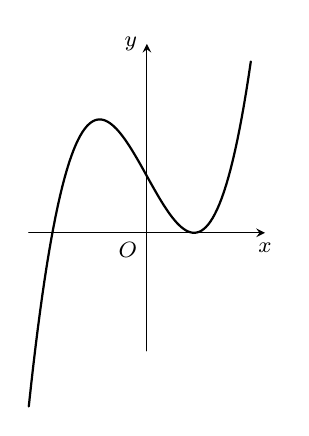
\begin{tikzpicture}[scale=0.6, font=\footnotesize, line join=round, line cap=round, >=stealth]
			\draw[->] (-2.5,0)--(2.5,0) node[below] {$x$};
			\draw[->] (0,-2.5)--(0,4) node[left] {$y$};
			\draw (0,0) node[below left] {$O$};
			\draw[thick, samples=100, domain=-2.5:2.2] plot (\x, {0.6*(\x+2)*(\x-1)^2});
		\end{tikzpicture}
	\end{center}
	Khẳng định nào sau đây là đúng?
	\choice
	{$a>0$, $b>0$, $c<0$}
	{$a>0$, $d<0$}
	{\True $a>0$, $d>0$}
	{$a>0$, $c>0$}
	\loigiai{Từ đồ thị ta có
		\begin{itemize}
			\item Nhánh cuối của đồ thị đi lên nên hệ số $a>0$.
			\item Đồ thị cắt trục tung $Oy$ tại điểm có tung độ dương, mà tại $x=0$ thì $y=d$. Suy ra $d>0$.
		\end{itemize}
		Vậy $a>0$, $d>0$.
	}
\end{ex}

\begin{ex}%[2D4H2-2]
	Cho hàm số $y=f(x)$ liên tục trên $[-1;3]$ thỏa mãn $\displaystyle\int\limits_{-1}^3 f(x)\mathrm{\,d}x=2$. Tích phân $\displaystyle\int\limits_{-1}^3 \left(3x^2+f(x)\right)\mathrm{\,d}x$ bằng
	\choice
	{$32$}
	{$12$}
	{$35$}
	{\True $30$}
	\loigiai{
		Ta có
		$\displaystyle\int\limits_{-1}^3\left(3x^2+f(x)\right)\mathrm{\,d}x=\int\limits_{-1}^3 3x^2\mathrm{\,d}x +\int\limits_{-1}^3 f(x)\mathrm{\,d}x=28+2=30$.}
\end{ex}

\begin{ex}%[2D4N1-3]
	Một nguyên hàm của hàm số $f(x)=\sin x$ là
	\choice
	{$F(x)=\cos x$}
	{$F(x)=\cos 2x$}
	{\True $F(x)=-\cos x$}
	{$F(x)=\dfrac{1}{2}\sin x$}
	\loigiai{
		Ta có $\displaystyle\int\limits\sin x\mathrm{\,d}x=-\cos x+C$.\\
		Với $C=0$, ta có một nguyên hàm của hàm số $f(x)=\sin x$ là $F(x)=-\cos x$.
	}
\end{ex}

\begin{ex}%[2H2N2-2]
	Trong không gian $Oxyz$, cho hai điểm $A(1;-2;1)$ và $B(2;3;-4)$. Tọa độ trung điểm $I$ của đoạn thẳng $AB$ là
	\choice
	{$I(3;1;-3)$}
	{$I\left(\dfrac{1}{2};\dfrac{5}{2};-\dfrac{5}{2}\right)$}
	{\True $I\left(\dfrac{3}{2};\dfrac{1}{2};-\dfrac{3}{2}\right)$}
	{$I\left(-\dfrac{1}{2};-\dfrac{5}{2};\dfrac{5}{2}\right)$}
	\loigiai{
		Do $I$ là trung điểm của đoạn thẳng $AB$ nên 
		$\heva{&x_I=\dfrac{x_A+x_B}{2}=\dfrac{3}{2}\\&y_I=\dfrac{y_A+y_B}{2}=\dfrac{1}{2}\\&z_I=\dfrac{z_A+z_B}{2}=-\dfrac{3}{2}}\Rightarrow I\left(\dfrac{3}{2};\dfrac{1}{2};-\dfrac{3}{2}\right)$.
	}
\end{ex}

\begin{ex}%[2H5H2-5]
	Trong không gian $Oxyz$, cho mặt phẳng $(P)\colon x-2y+z-1=0$ và đường thẳng $d\colon\dfrac{x-1}{2}=\dfrac{y+1}{-1}=\dfrac{z}{1}$. Kết luận nào sau đây là đúng?
	\choice
	{$d\parallel (P)$}
	{$d\subset (P)$}
	{\True $d$ và $(P)$ có $1$ điểm chung}
	{$d\perp (P)$}
	\loigiai{
		Mặt phẳng $(P)$ có vectơ pháp tuyến $\overrightarrow{n}=(1;-2;1)$.\\
		Đường thẳng $d$ có vectơ chỉ phương $\overrightarrow{u}=(2;-1;1)$ và đi qua điểm $M(1;-1;0)$.\\
		Ta có $\overrightarrow{n}\cdot\overrightarrow{u}=1\cdot 2+(-2)\cdot (-1)+1\cdot 1=2+2+1=5\neq 0$ và $\overrightarrow{n}$ không cùng phương với $\overrightarrow{u}$.\\
		Vậy đường thẳng $d$ cắt mặt phẳng $(P)$ và $d$ không vuông góc với $(P)$.
	}
\end{ex}

\begin{ex}%[1D6H2-2]
	Cho các số thực $x$ và $y$. Với $x>0$ thì đẳng thức nào sau đây đúng?
	\choice
	{\True $\log_5\dfrac{x}{5^y}=\log_5 x-y$}
	{$\log(xy^4)=\log x+4\log |y|$}
	{$\ln(xy^2)=\ln x+2\ln y$}
	{$\log_2 (x+2y)=\log_2 x+\log_2 2y$}
	\loigiai{Khi $x>0$, ta có $\log_5\dfrac{x}{5^y}=\log_5 x-\log_5 5^y=\log_5 x-y$ đúng với mọi $y$.}
\end{ex}

\begin{ex}%[2H5N3-3]
	Trong không gian $Oxyz$, mặt cầu $(S)$ có tâm $I(1;2;-3)$, đi qua điểm $M(2;4;-1)$ có phương trình là
	\choice
	{\True $(x-1)^2+(y-2)^2+(z+3)^2=9$}
	{$(x+1)^2+(y+2)^2+(z-3)^2=3$}
	{$(x+1)^2+(y+2)^2+(z-3)^2=9$}
	{$(x-1)^2+(y-2)^2+(z+3)^2=3$}
	\loigiai{
		Bán kính mặt cầu $R=IM=\sqrt{(2-1)^2+(4-2)^2+(-1-(-3))^2}=3$.\\
		Phương trình mặt cầu tâm $I(1;2;-3)$ và bán kính $R=3$ là
		$$(x-1)^2+(y-2)^2+(z+3)^2=3^2\Leftrightarrow (x-1)^2+(y-2)^2+(z+3)^2=9.$$
	}
\end{ex}
\Closesolutionfile{ans}
\cauds
\Opensolutionfile{ans}[ans/De37-P2]
\begin{ex}%[0D0H2-9]
	Tại một tổ bầu cử Quốc hội khóa $XVI$ của phường Yên Hòa có $5$ ứng cử viên trong đó có ông A và ông B. Kết quả kiểm phiếu của $1\,500$ cử tri cho thấy:
	\begin{itemize}
		\item Có $900$ cử tri bầu cho ông A.
		\item Có $800$ cử tri bầu cho ông B.
		\item Có $200$ cử tri không bầu cho cả ông A và ông B.
	\end{itemize}
	Biết rằng mỗi cử tri có thể chọn một trong hai ứng cử viên hoặc chọn cả hai hoặc không chọn ai trong hai ứng cử viên $A, B$.
	\choiceTF
	{\True Số cử tri bỏ phiếu chọn cả hai ứng cử viên $A, B$ là $400$}
	{Xác suất để chọn một cử tri trong số $1\,500$ cử tri nói trên bầu cho cả hai ông $A, B$ là $\dfrac{8}{15}$}
	{\True Xác suất để chọn một cử tri trong số $1\,500$ cử tri nói trên chỉ bầu cho ông A là $\dfrac{1}{3}$}
	{\True Nếu chọn một cử tri đã bầu cho ứng cử viên A trong số $1\,500$ cử tri nói trên, xác suất để người đó không bầu cho ứng cử viên B là $\dfrac{5}{9}$}
	\loigiai{
		\begin{itemchoice}
			\itemch Gọi A là tập hợp các cử tri bầu cho ông A, B là tập hợp các cử tri bầu cho ông B.\\
			Số cử tri bầu cho ít nhất một trong hai ông A hoặc B là $n(A\cup B)=1\,500-200=1\,300$.\\
			Số cử tri bầu cho cả hai ông A và B là $n(A\cap B)=n(A)+n(B)-n(A\cup B)=900+800-1\,300=400$.
			\itemch Xác suất để chọn một cử tri bầu cho cả hai ông A, B là $\mathrm{P}(A\cap B)=\dfrac{n(A\cap B)}{n(\Omega)}=\dfrac{400}{1\,500}=\dfrac{4}{15}$.
			\itemch Số cử tri chỉ bầu cho ông A là $n(A\setminus B)=n(A)-n(A\cap B)=900-400=500$.\\
			Xác suất để chọn một cử tri chỉ bầu cho ông A là $\mathrm{P}(A\setminus B)=\dfrac{500}{1\,500}=\dfrac{1}{3}$.
			\itemch Trong số $900$ cử tri đã bầu cho ông A, số người không bầu cho ông B chính là số người chỉ bầu cho ông A, bằng $500$.\\
			Xác suất cần tìm là $P=\dfrac{500}{900}=\dfrac{5}{9}$.
		\end{itemchoice}
	}
\end{ex}

\begin{ex}%[0D2V2-3]
	Một xí nghiệp sản xuất hai loại sản phẩm I và II. Mỗi kilôgam sản phẩm loại I cần $2$ kg nguyên liệu và $30$ giờ làm, đem lại mức lợi nhuận $400$ nghìn đồng. Mỗi kilôgam sản phẩm loại II cần $4$ kg nguyên liệu và $15$ giờ làm, đem lại mức lợi nhuận $300$ nghìn đồng. Xí nghiệp có $200$ kg nguyên liệu và tối đa $1\,200$ giờ làm việc. Gọi $x, y$ lần lượt là số kg sản phẩm loại I và loại II xí nghiệp sản xuất.
	\choiceTF
	{\True Số kg nguyên liệu xí nghiệp cần dùng để sản xuất $x$ (kg) sản phẩm loại I và $y$ (kg) sản phẩm loại II là $2x+4y$ (kg)}
	{Số giờ làm xí nghiệp cần để sản xuất $x$ (kg) sản phẩm loại I và $y$ (kg) sản phẩm loại II là $2x+y$ (giờ làm)}
	{\True Nếu xí nghiệp sản xuất $5$ (kg) sản phẩm loại I và $6$ (kg) sản phẩm loại II thì xí nghiệp có lợi nhuận là $3\,800$ nghìn đồng}
	{Lợi nhuận tối đa xí nghiệp có được là $12\,000$ nghìn đồng}
	\loigiai{
		\begin{itemchoice}
			\itemch Mỗi kg loại I cần $2$ kg nguyên liệu, mỗi kg loại II cần $4$ kg nguyên liệu. Vậy tổng lượng nguyên liệu là $2x+4y$ (kg).
			\itemch Mỗi kg loại I cần $30$ giờ làm, mỗi kg loại II cần $15$ giờ làm. Vậy tổng số giờ làm là $30x+15y$ (giờ).
			\itemch Lợi nhuận thu được với $x$ (kg) sản phằm loại I và $y$ (kg) sản phẩm loại II là $F(x;y)=400x+300y$.\\
			Với $x=5$, $y=6$ ta có $F(5;6)=400\cdot 5+300\cdot 6=2\,000+1\,800=3\,800$ nghìn đồng.
			\itemch Tìm giá trị lớn nhất của $F(x;y)=400x+300y$ với hệ điều kiện:
			$$\heva{&x\ge 0, y\ge 0\\&2x+4y\le 200\Leftrightarrow x+2y\le 100\\&30x+15y\le 1\,200\Leftrightarrow 2x+y\le 80.}$$
			\begin{center}
				\begin{tikzpicture}[line join=round, line cap=round,>=stealth,thick,scale=0.2]
						\tikzset{every node/.style={scale=0.9}}
						\begin{scope}
							\clip (-1,-1) rectangle (50,60);
							\fill[pattern=north east lines] (0,-1)--(-1,-1)--(-1,60)--(0,60)--cycle;
							\fill[pattern=north east lines] (-1,0)--(-1,-1)--(50,-1)--(50,0)--cycle;
							\fill[pattern=north east lines] (-21,60.5)--(103,60.5)--(103,-1.5)--cycle;
							\fill[pattern=north east lines] (-2,84)--(51,84)--(51,-22)--cycle;
							\draw (-20,60)--(102,-1);
							\draw (10,60)--(40.5,-1);
						\end{scope}
						\draw[->] (-1,0)--(50,0) node[below]{$x$};
						\draw[->] (0,-1)--(0,60) node[left]{$y$};
						\fill (0,0)node[shift={(-135:2.5mm)}]{\footnotesize{$O$}}circle(1.2pt) (40,0)node[below]{\footnotesize{$A$}}circle(1.2pt) (0,50)node[left]{\footnotesize{$C$}}circle(1.2pt) (20,40)node[above right]{\footnotesize{$B$}}circle(1.2pt);
					\end{tikzpicture}
			\end{center}
			Các đỉnh của miền nghiệm là $O(0;0)$, $A(40;0)$, $B(20;40)$, $C(0;50)$.\\
			Ta có $F(0;0)=0$; $F(40;0)=16\,000$; $F(20;40)=20\,000$; $F(0;50)=15\,000$.\\
			Vậy lợi nhuận tối đa là $20\,000$ nghìn đồng.
		\end{itemchoice}
	}
\end{ex}

\begin{ex}%[2D4V1-2]
	Cho hàm số $y=f(x)=\dfrac{x^2-3x+5}{x+1}$. Giả sử đồ thị hàm số $y=f(x)$ có hai điểm cực trị là $A$ và $B$.
	\choiceTF
	{\True Tiệm cận đứng của đồ thị hàm số $y=f(x)$ là đường thẳng $x=-1$}
	{\True Đạo hàm của hàm số $y=f(x)$ là $f'(x)=\dfrac{x^2+2x-8}{(x+1)^2},\forall x\neq -1$}
	{Hai điểm $A$ và $B$ nằm về hai phía của trục hoành và $AB=5\sqrt{17}$}
	{Gọi $y=g(x)$ là một nguyên hàm của hàm số $f'(x)$ thỏa mãn $g(0)=12$. Giả sử $C, D$ là hai điểm cực trị của đồ thị hàm số $y=g(x)$ thì $4$ điểm $A,B,C,D$ lập thành tứ giác có diện tích là $42$ (đơn vị diện tích)}
	\loigiai{
		\begin{itemchoice}
			\itemch Ta có $\lim\limits_{x\to -1^+} f(x)=+\infty$ nên đường thẳng $x=-1$ là tiệm cận đứng của đồ thị hàm số.
			\itemch Ta có $f'(x)=\dfrac{x^2+2x-8}{(x+1)^2}$ $\forall x\ne-1$.
			\itemch Ta có $f'(x)=0\Leftrightarrow x^2+2x-8=0\Leftrightarrow x=2$ hoặc $x=-4$.\\
			Suy ra hai điểm cực trị của đồ thị hàm số là  $A(2;1)$ và $B(-4;-11)$.\\
			Do $y_A$ và $y_B$ trái dấu nên $A$ và $B$ nằm về hai phía trục hoành.\\
			Mặt khác ta có $AB=\sqrt{(-4-2)^2+(-11-1)^2}=\sqrt{36+144}=\sqrt{180}=6\sqrt{5}$.
			\itemch Vì $g(x)$ là nguyên hàm của $f'(x)$ nên $g(x)=f(x)+C$.\\
			Ta có $g(0)=12\Rightarrow f(0)+C=12\Rightarrow 5+C=12\Rightarrow C=7$.\\
			Vậy $g(x)=\dfrac{x^2-3x+5}{x+1}+7$. Đồ thị $g(x)$ là đồ thị $f(x)$ tịnh tiến lên trên $7$ đơn vị.\\
			Các điểm cực trị của $g(x)$ là $C(2;8)$ và $D(-4;-4)$.\\
			Dễ thấy $ABCD$ tạo thành hình bình hành nên có diện tích là $S=2\cdot S_{ABC}=AC\cdot |x_A-x_B|=7\cdot 6=42$.
		\end{itemchoice}
	}
\end{ex}

\begin{ex}%[2H5H2-5]
	Trong không gian $Oxyz$, cho điểm $A(1;1;1)$, điểm $B(-1;2;0)$, đường thẳng $\Delta\colon\dfrac{x-1}{2}=\dfrac{y+1}{-2}=\dfrac{z-3}{1}$ và mặt phẳng $(P)\colon x-2y-2z+15=0$.
	\choiceTF
	{\True Một véc-tơ chỉ phương của đường thẳng $\Delta$ là $\overrightarrow{u}=(-2;2;-1)$}
	{\True Nếu góc giữa đường thẳng $\Delta$ và mặt phẳng $(P)$ là $\varphi$ thì $\sin\varphi=\dfrac{2}{9}$}
	{Gọi $(Q)$ là mặt phẳng chứa các điểm $A, B$ và song song với $\Delta$. Nếu mặt phẳng $(Q)$ cắt mặt phẳng $(P)$ theo giao tuyến là $d$ thì đường thẳng $d$ đi qua điểm $E(-1;2;5)$}
	{\True Nếu giao điểm của đường thẳng $\Delta$ và mặt phẳng $(P)$ là điểm $I(a;b;c)$ thì $a+2b+c=5$}
	\loigiai{
		\begin{itemchoice}
			\itemch Đường thẳng $\Delta$ có VTCP $\overrightarrow{u}_{\Delta}=(2;-2;1)$. Véc-tơ $\overrightarrow{u}=(-2;2;-1)=-\overrightarrow{u}_{\Delta}$ cũng là một VTCP của $\Delta$.
			\itemch Mặt phẳng $(P)$ có VTPT $\overrightarrow{n}=(1;-2;-2)$.\\
			$$\sin\varphi=\dfrac{|\overrightarrow{u}_{\Delta}\cdot\overrightarrow{n}|}{|\overrightarrow{u}_{\Delta}|\cdot |\overrightarrow{n}|}=\dfrac{|2\cdot 1+(-2)\cdot (-2)+1\cdot (-2)|}{\sqrt{2^2+(-2)^2+1^2}\cdot\sqrt{1^2+(-2)^2+(-2)^2}}=\dfrac{|2+4-2|}{3\cdot 3}=\dfrac{4}{9}.$$
			\itemch Ta có $\overrightarrow{AB}=(-2;1;-1)$. Mặt phẳng $(Q)$ có một VTPT là $\overrightarrow{n}_Q=\left[\overrightarrow{AB},\overrightarrow{u}_{\Delta}\right]=(1;0;-2)$.\\
			Phương trình $(Q)\colon 1(x-1)+0(y-1)-2(z-1)=0\Leftrightarrow x-2z+1=0$.\\
			Tạp hợp các điểm thuộc giao tuyến $d$ thỏa mãn hệ phương trình $\heva{&x-2z+1=0\\&x-2y-2z+15=0.}$\\
			Thay $E(-1;2;5)$ vào hệ ta thấy không thỏa nên $E\notin d$.
			\itemch Ta có $I\in\Delta\Rightarrow I(1+2t; -1-2t; 3+t)$.\\
			$I\in (P)\Rightarrow (1+2t)-2(-1-2t)-2(3+t)+15=0\Leftrightarrow 4t+12=0\Leftrightarrow t=-3$.\\
			Vậy $\Delta$ cắt $(P)$ tại điểm $I(-5;5;0)$, suy ra $a=-5$, $b=5$, $c=0$ nên $a+2b+c=-5+10+0=5$.
		\end{itemchoice}
	}
\end{ex}
\Closesolutionfile{ans}
\caukq
\Opensolutionfile{ans}[ans/De37-P3]
\begin{ex}%[2D4V3-2]
	Dự án \lq\lq Công viên Thiên văn học\rq\rq\ được khởi công năm 2017 do Tập đoàn Nam Cường đầu tư và đưa vào sử dụng từ đầu năm 2024. Để tạo điểm nhấn, các kỹ sư đã thiết kế một con đường và Vọng Lâu giữa hồ. Theo một tỉ lệ nhất định, con đường ở giữa công viên được mô phỏng như hình vẽ, biết rằng trên hệ trục tọa độ tương ứng của hình vẽ thì:
	\begin{itemize}
		\item Các đường cong $BC$, $FG$ là $2$ phần của Parabol có phương trình $y=f(x)=0{,}11x^2+1$.
		\item Các đường cong $AQ$, $PK$ là $2$ phần của Parabol có phương trình $y=g(x)=0{,}1x^2+0{,}41$.
		\item Đường cong qua $3$ điểm $Q$, $O$, $P$ là một phần của Parabol có phương trình là $y=h(x)=0{,}13x^2$.
		\item Các điểm $C$, $D$ có cùng hoành độ là $-0{,}35$. Các điểm $E$, $F$ có cùng hoành độ là $0{,}35$.
		\item Các điểm $D$, $E$ có cùng tung độ là $2{,}65$.
		\item Các điểm $A$, $Q$, $P$, $K$ có hoành độ lần lượt là $-6$; $-\sqrt{14}$; $\sqrt{14}$; $6$.
		\item Điểm $B$, $G$ có hoành độ lần lượt là $-5{,}7$ và $5{,}7$.
	\end{itemize}
	\begin{center}
		\begin{tikzpicture}[>=stealth,line join=round,line cap=round,font=\footnotesize,scale=0.85,xscale=1.2]
			\draw[->] (-7,0)--(7,0) node[right] {$x$};
			\draw[->] (0,-1)--(0,5) node[above] {$y$};
			\draw
			[smooth,domain=-6:{-sqrt(14)},samples=100]plot(\x,{0.1*(\x)^2+0.41})
			[smooth,domain={sqrt(14)}:6,samples=100]plot(\x,{0.1*(\x)^2+0.41})
			[smooth,domain={-sqrt(14)}:{sqrt(14)},samples=100]plot(\x,{0.13*(\x)^2})
			[smooth,domain=-5.7:-0.35,samples=100]plot(\x,{0.11*(\x)^2+1})
			[smooth,domain=0.35:5.7,samples=100]plot(\x,{0.11*(\x)^2+1})
			(-0.35,1.013475)--(-0.35,2.65)--(0.35,2.65)--(0.35,1.013475) (5.7,4.5739)--(6,4.01) (-5.7,4.5739)--(-6,4.01)
			;
			\draw[pattern=bricks](-6,4.01)--plot[smooth,domain=-6:{-sqrt(14)},samples=100](\x,{0.1*(\x)^2+0.41})--plot[smooth,domain={-sqrt(14)}:{sqrt(14)},samples=100](\x,{0.13*(\x)^2})--plot[smooth,domain={sqrt(14)}:6,samples=100](\x,{0.1*(\x)^2+0.41})--(5.7,4.5739)--plot[smooth,domain=5.7:0.35,samples=100](\x,{0.11*(\x)^2+1})--(0.35,2.65)--(-0.35,2.65)--(-0.35,1.013475)--plot[smooth,domain=-0.35:-5.7,samples=100](\x,{0.11*(\x)^2+1})--(-6,4.01);
			\draw[dashed] (-6,4.01)--(-6,0) (6,0)--(6,4.01) (-5.7,4.5739)--(5.7,4.5739) ({-sqrt(14)},0)--({-sqrt(14)},91/50) ({sqrt(14)},0)--({sqrt(14)},91/50);
			\fill (0,0)node[shift={(-135:2.5mm)}]{\footnotesize{$O$}}circle(1.2pt) (-6,4.01)node[below left=-2pt]{\footnotesize{$A$}}circle(1.2pt) (6,4.01)node[below right=-2pt]{\footnotesize{$K$}}circle(1.2pt) (-5.7,4.5739)node[above=-2pt]{\footnotesize{$B$}}circle(1.2pt) (5.7,4.5739)node[above=-2pt]{\footnotesize{$G$}}circle(1.2pt) (-0.35,1.013475)node[above left=-2pt]{\footnotesize{$C$}}circle(1.2pt) (0.35,1.013475)node[above right=-2pt]{\footnotesize{$F$}}circle(1.2pt) (-0.35,2.65)node[above left=-2pt]{\footnotesize{$D$}}circle(1.2pt) (0.35,2.65)node[above right=-2pt]{\footnotesize{$E$}}circle(1.2pt) (0.35,2.65)node[above right=-2pt]{\footnotesize{$E$}}circle(1.2pt)
			({sqrt(14)},91/50)node[below right=-2pt]{\footnotesize{$P$}}circle(1.2pt)
			({-sqrt(14)},91/50)node[below left=-2pt]{\footnotesize{$Q$}}circle(1.2pt) (-6,0)node[below=-2pt]{\footnotesize{$-6$}}circle(1.2pt) (6,0)node[below=-2pt]{\footnotesize{$6$}}circle(1.2pt) ({-sqrt(14)},0)node[below=-2pt]{\footnotesize{$-\sqrt{14}$}}circle(1.2pt) ({sqrt(14)},0)node[below=-2pt]{\footnotesize{$\sqrt{14}$}}circle(1.2pt);
		\end{tikzpicture}
	\end{center}
	Dựa theo số liệu ở mô tả, tính diện tích phần con đường được tô hình viên gạch trong hình vẽ (\textit{kết quả làm tròn đến hàng phần mười}).
	\par\shortans[oly]{24,6}
	\loigiai{Xét phần hình vẽ bên phải trục $Oy$, ta có
		\begin{itemize}
			\item Trong miền $0\le x\le0{,}35$, diện tích cần tìm là $S_1=\displaystyle\int\limits_0^{0{,35}}\left(2{,}65-0{,}13x^2\right)\mathrm{\,d}x$.
			\item Trong miền $0{,}35\le x\le\sqrt{14}$, diện tích cần tìm là $S_2=\displaystyle\int\limits_{0{,35}}^{\sqrt{14}}\left(0{,}11x^2+1-0{,}13x^2\right)\mathrm{\,d}x$.
			\item Trong miền $\sqrt{14}\le x\le5{,}7$, diện tích cần tìm là $S_3=\displaystyle\int\limits_{\sqrt{14}}^{5{,}7}\left(0{,}11x^2+1-0{,}1x^2-0{,}41\right)\mathrm{\,d}x$.
			\item Trong miền $5{,}7\le x\le6$.\\
			Ta có $G(5{,}7;4{,}5739)$ và $K(6;4{,}01)$ nên phương trình đường thẳng $GK$ là $y=-\dfrac{5\,639}{3\,000}x+\dfrac{1\,911}{125}$.\\
			Diện tích cần tìm là $S_4=\displaystyle\int\limits_{5{,}7}^6\left(-\dfrac{5\,639}{3\,000}x+\dfrac{1\,911}{125}-0{,}1x^2-0{,}41\right)\mathrm{\,d}x$.
		\end{itemize}
		Diện tích phần cần tính là $S=2\left(S_1+S_2+S_3+S_4\right)\approx24{,}6$.}
\end{ex}

\begin{ex}%[2D1V5-8]
	Máng trượt nước cao nhất thế giới là máng trượt \lq\lq Verruckt\rq\rq\ trong công viên nước \lq\lq Schlitterbahn – MỸ\rq\rq. Máng trượt này có độ cao từ đỉnh khoảng $50$\,m so với mặt đất. Gắn vào hệ trục $Oxy$ với một đơn vị là $10$\,m thì hình ảnh máng trượt được mô phỏng là hình ảnh của một đồ thị hàm bậc ba có dạng $y=f(x)=ax^3+bx^2+cx+d$ như hình vẽ.
	\begin{center}
		\begin{tikzpicture}[>=stealth,line join=round,line cap=round,font=\footnotesize,scale=0.75]
			\draw[->] (-1,0)--(16,0) node[right] {$x$};
			\draw[->] (0,-1)--(0,6) node[above] {$y$};
			\draw [smooth,domain=0:15.2,samples=100]plot(\x,{-0.013*(\x)^3+0.33*(\x)^2-2.325*(\x)+5});
			\draw[dashed,thick] (1.5,0)--(1.5,2.211125) (3,0)--(3,{161/250}) (7,0)--(7,{109/250}) (8.5,0)--(8.5,{8771/8000}) (10,0)--(10,7/4) (11.25,0)--(11.25,1075/512) (12.5,0)--(12.5,135/64) (13.75,0)--(13.75,833/512) (15,0)--(15,1/2);
			\fill (0,0)node[shift={(-135:2.5mm)}]{\footnotesize{$O$}}circle(1.2pt) (1.5,0)node[below=-2pt]{\footnotesize{$1{,}5$}}circle(1.2pt) (3,0)node[below=-2pt]{\footnotesize{$3$}}circle(1.2pt) (5,0)node[below=-2pt]{\footnotesize{$5$}}circle(1.2pt) (7,0)node[below=-2pt]{\footnotesize{$7$}}circle(1.2pt) (8.5,0)node[below=-2pt]{\footnotesize{$8{,}5$}}circle(1.2pt) (10,0)node[below=-2pt]{\footnotesize{$10$}}circle(1.2pt) (11.25,0)node[below=-2pt]{\footnotesize{$11{,}25$}}circle(1.2pt) (12.5,0)node[below=-2pt]{\footnotesize{$12{,}5$}}circle(1.2pt) (13.75,0)node[below=-2pt]{\footnotesize{$13{,}75$}}circle(1.2pt) (15,0)node[below=-2pt]{\footnotesize{$15$}}circle(1.2pt) (0,5)node[left=-2pt]{\footnotesize{$5$}}circle(1.2pt);
		\end{tikzpicture}
	\end{center}
	Điểm $B(5;0)$ là điểm cực tiểu của đồ thị hàm số $y=f(x)$, đồ thị cắt trục tung tại điểm $A$ có tung độ bằng $5$ và đi qua điểm $C\left(15;\dfrac{1}{2}\right)$. Tại các điểm có hoành độ lần lượt là $1{,}5$; $3$; $7$; $8{,}5$; $10$; $11{,}25$; $12{,}5$; $13{,}75$; $15$ các kỹ sư thiết kế các cột đỡ cho cây cầu (cột đỡ là các đường nét đứt như \textit{hình 6}, biết các đường đó vuông góc với $Ox$). Tính tổng chiều cao của các cột đỡ theo tỉ lệ đã cho trong \textit{hình 6} ( \textit{kết quả làm tròn đến hàng phần mười}).
	\par\shortans[oly]{12,5}
	\loigiai{
		Hàm số bậc ba $y=ax^3+bx^2+cx+d$.
		\begin{itemize}
			\item Đồ thị cắt trục tung tại $(0;5)\Rightarrow d=5$.
			\item Điểm cực tiểu $B(5;0)$ nên $f(5)=0$ và $f'(5)=0$.
			\item Đồ thị đi qua $C\left(15;\dfrac{1}{2}\right)\Rightarrow f(15)=0{,}5$.
		\end{itemize}
		Ta có hệ phương trình:
		$\heva{&125a+25b+5c+5=0\\&75a+10b+c=0\\&3375a+225b+15c+5=0{,}5}\Leftrightarrow\heva{&a=-\dfrac{13}{1\,000}\\&b=\dfrac{33}{100}\\&c=-\dfrac{93}{40}}$.\\
		Vậy $f(x)=-\dfrac{13}{1\,000}x^3+\dfrac{33}{100}x^2-\dfrac{93}{40}x+5$.\\
		Tổng chiều cao các cột đỡ là
		$$L=f(1{,}5)+f(3)+f(7)+f(8{,}5)+f(10)+f(11{,}25)+f(12{,}5)+f(13{,}75)+f(15)=\dfrac{7\,983}{640}\approx 12{,}5\text{\,(m).}$$
	}
\end{ex}

\begin{ex}%[2H5V3-4]
	Trong không gian $Oxyz$, cho mặt cầu $(S)\colon (x-2)^2+(y-1)^2+(z-3)^2=9$ và hai điểm $A(1;1;3)$, $B(21;9;-13)$. Giả sử điểm $M(a;b;c)$ thuộc mặt cầu $(S)$ sao cho $3MA^2+MB^2$ đạt giá trị nhỏ nhất. Khi đó giá trị của biểu thức $T=a\cdot b\cdot c$ bằng bao nhiêu?
	\par\shortans[oly]{8}
	\loigiai{\begin{center}
			\begin{tikzpicture}[>=stealth,line join=round,line cap=round,font=\footnotesize,scale=0.5]
				\path (0,0) coordinate (I)
				(4,3) coordinate (M_0)
				(5,0) coordinate (M)
				($(I)!2!(M_0)$) coordinate (G)
				;
				\draw 
				(I)circle(5)
				(M)--(G)--(M_0)
				;
				\draw[dashed] (M)--(I)--(M_0);
				\foreach \p / \r in {I/135,G/45,M/-45,M_0/90}
				\fill (\p) circle (1.2pt) node[shift={(\r:3mm)}]{$\p$};
			\end{tikzpicture}
		\end{center}
		Mặt cầu $(S)$ có tâm $I(2;1;3)$ và bán kính $R=3$.\\
		Gọi $G$ là điểm thỏa mãn $3\overrightarrow{GA} +\overrightarrow{GB}=\overrightarrow{0}\Rightarrow\heva{&x_G=\dfrac{3x_A+x_B}{4}=6\\&y_G=\dfrac{3y_A+y_B}{4}=3\\&z_G=\dfrac{3z_A+z_B}{4}=-1}\Rightarrow G(6;3;-1)$.\\
		Ta có 
		\begin{align*}
			3MA^2+MB^2&=3\overrightarrow{MA}^2 +\overrightarrow{MB}^2=3\left(\overrightarrow{MG} +\overrightarrow{GA}\right)^2+\left(\overrightarrow{MG} +\overrightarrow{GB}\right)^2\\
			&= 4MG^2+2\overrightarrow{MG}\left(3\overrightarrow{GA} +\overrightarrow{GB}\right)+3GA^2+GB^2=4MG^2+3GA^2+GB^2.
		\end{align*}
		Do $A$, $B$, $G$ cố định nên biểu thức nhỏ nhất khi $MG$ nhỏ nhất.\\
		Vì $M\in (S)$ nên $M$ là giao điểm của đoạn thẳng $IG$ với mặt cầu $(S)$.\\
		Ta có $\overrightarrow{IG}=(4;2;-4)\Rightarrow IG=6 > R$.\\
		Điểm $M$ thỏa mãn $\overrightarrow{IM}=\dfrac{R}{IG}\overrightarrow{IG}=\dfrac{3}{6}\overrightarrow{IG}=\dfrac{1}{2}\overrightarrow{IG}\Rightarrow M(4; 2; 1)$.\\
		Vậy $T=a\cdot b\cdot c=4\cdot 2\cdot 1=8$.
	}
\end{ex}
\begin{ex}%[1D9V1-3]
	Cho một hình bát giác đều có tám đỉnh $A$, $B$, $C$, $D$, $E$, $F$, $G$, $H$. Người ta gắn ngẫu nhiên vào $8$ đỉnh này $8$ số tự nhiên $1$, $2$, $3$, $4$, $5$, $6$, $7$, $8$ (mỗi đỉnh gắn một số). Chọn ngẫu nhiên một tam giác có $3$ đỉnh lấy từ $8$ đỉnh của bát giác đã cho. Gọi $P$ là xác suất để thu được một tam giác vuông với $3$ số trên $3$ đỉnh của tam giác đó lập thành một cấp số cộng. Biết $P=\dfrac{m}{n}$ (phân số tối giản). Tính $m+3n$.	
	\par\shortans[oly]{303}
	\loigiai{\begin{center}
			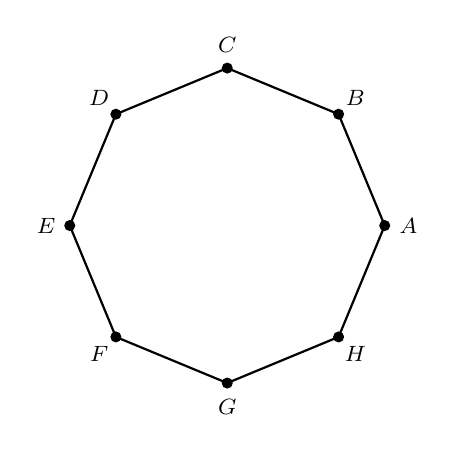
\begin{tikzpicture}[scale=1, font=\footnotesize, line join=round, line cap=round, >=stealth]
				\foreach \i/\l in {0/A, 45/B, 90/C, 135/D, 180/E, 225/F, 270/G, 315/H}
				\draw (\i:2) coordinate (\l);
				\draw[thick] (A)--(B)--(C)--(D)--(E)--(F)--(G)--(H)--cycle;
				\foreach \p in {A,B,C,D,E,F,G,H} \fill (\p) circle (2pt);
				\foreach \i/\l in {0/A, 45/B, 90/C, 135/D, 180/E, 225/F, 270/G, 315/H}
				\node at (\i:2.3) {$\l$};
			\end{tikzpicture}
		\end{center}
	Xét biến cố $A\colon$ ``tam giác được chọn ngẫu nhiên là một tam giác vuông'', ta có 
		\begin{itemize}
			\item Số cách chọn $1$ tam giác bất kỳ từ $8$ đỉnh là: $\mathrm{C}_8^3=56$ cách.
			\item Để tam giác chọn ra là tam giác vuông thì cạnh huyền của nó phải là đường kính của đường tròn ngoại tiếp bát giác đều. Hình bát giác đều có $4$ đường kính nối các đỉnh đối diện: $(A,E), (B,F), (C,G), (D,H)$. 
			\item Với mỗi đường kính, chọn thêm $1$ trong $6$ đỉnh còn lại ta sẽ được một tam giác vuông. Do đó số tam giác vuông tạo thành là: $4 \cdot 6=24$ tam giác.
			\item Suy ra: $\mathrm{P}(A)=\dfrac{24}{56}=\dfrac{3}{7}$.
		\end{itemize}
	Xét biến cố $B\colon$ ``$3$ số gán trên $3$ đỉnh của một tam giác bất kỳ lập thành một cấp số cộng'', ta có
		\begin{itemize}
			\item Chọn $3$ số ngẫu nhiên từ tập $\{1;2;3;4;5;6;7;8\}$ để đặt vào $3$ đỉnh của tam giác có $\mathrm{C}_8^3=56$ cách.
			\item Các bộ $3$ số phân biệt $\{a,b,c\}$ lập thành một cấp số cộng gồm có:
			\begin{itemize}
				\item Công sai $d=1$: $\{1;2;3\}$, $\{2;3;4\}$, $\{3;4;5\}$, $\{4;5;6\}$, $\{5;6;7\}$, $\{6;7;8\}$ $\rightarrow$ có $6$ bộ.
				\item Công sai $d=2$: $\{1;3;5\}$, $\{2;4;6\}$, $\{3;5;7\}$, $\{4;6;8\}$ $\rightarrow$ có $4$ bộ.
				\item Công sai $d=3$: $\{1;4;7\}$, $\{2;5;8\}$ $\rightarrow$ có $2$ bộ.
			\end{itemize}
			Tổng số bộ thỏa mãn là: $6+4+2=12$ bộ.
			\item Suy ra: $\mathrm{P}(B)= \dfrac{12}{56}=\dfrac{3}{14}$.
		\end{itemize}
		Xác suất cần tìm là $\mathrm{P}(AB)=\mathrm{P}(A)\cdot\mathrm{P}(B)=\dfrac{3}{7} \cdot \dfrac{3}{14}=\dfrac{9}{98}$.\\
		Suy ra $m=9$ và $n=98$. \\
		Vậy giá trị của biểu thức cần tìm là: $m+3n=9+3 \cdot 98=303$.}
\end{ex}

\begin{ex}%[1D6V3-5]
	Thị trường chứng khoán là một kênh huy động vốn hiệu quả cho các doanh nghiệp và nền kinh tế. Ở Việt Nam, một phiên giao dịch được tính từ lúc $9$ giờ $00$ sáng đến lúc đóng cửa lúc $14$ giờ $30$ cùng ngày, thị trường có $1{,}5$ tiếng nghỉ trưa. Trong mỗi phiên giao dịch, giá mở cửa của một cổ phiếu gọi là \textit{giá tham chiếu} (là giá đóng cửa của phiên hôm trước). Phiên giao dịch ngày $1$ tháng $3$ năm 2026 với những tin tức tích cực, cổ phiếu của công ty \lq\lq Công ty Cổ phần Lọc hóa dầu Bình Sơn\rq\rq\ mã chứng khoán $BSR$, phiên giao dịch ngày $1$ tháng $3$ và $2$ phiên giao dịch tiếp theo, mã này tăng trần (tăng tối đa $7\%$). Hai phiên giao dịch tiếp theo giá cổ phiếu $BSR$ tăng lần lượt là $4\%$ và $4{,}5\%$. Tuy nhiên sau đó, tình hình Thế giới tác động ngược lại nên mã cổ phiếu này lại bị bán tháo dẫn đến giảm sàn trong $2$ phiên tiếp theo (giảm tối đa $7\%$ trong phiên giao dịch). 
	Giá tăng hay giảm của một cổ phiếu trong một phiên được tính theo công thức:
	$$\text{Mức tăng (giảm)}=\dfrac{\text{Giá đóng cửa} -\text{Giá tham chiếu}}{\text{Giá tham chiếu}}$$
	Biết được thông tin trên, ông An - một nhà đầu tư kì cựu - ngay từ đầu phiên ngày $1$ tháng $3$ đã mua được $15\,000$ cổ phiếu $BSR$ với mức giá tham chiếu $31{,}5$ (đơn vị: nghìn đồng). Hỏi sau $7$ phiên giao dịch tính từ ngày $1$ tháng $3$ thì ông An đã có lợi nhuận là bao nhiêu triệu đồng? (\textit{Kết quả làm tròn đến hàng đơn vị}).
	\par\shortans[oly]{42}
	\loigiai{
		Gọi $P_0=31{,}5$ là giá tham chiếu ngày đầu tiên (đơn vị: nghìn đồng).\\
		Từ công thức giả thiết, ta có
		\begin{eqnarray*}
			&&\text{Mức tăng (giảm)}=\dfrac{\text{Giá đóng cửa} - \text{Giá tham chiếu}}{\text{Giá tham chiếu}}\\
			&\Rightarrow&\text{Giá đóng cửa}=\text{Giá tham chiếu} \cdot [1+\text{Mức tăng (giảm)}].
		\end{eqnarray*}
		Từ đó suy ra diễn biến giá cổ phiếu $BSR$ qua $7$ phiên như sau:
		\begin{itemize}
			\item Phiên 1, 2, 3 (tăng trần $7\%$): Giá sau phiên 3 là $P_3=P_0\cdot (1+7\%)^3$.
			\item Phiên 4 (tăng $4\%$): Giá sau phiên 4 là $P_4=P_3\cdot (1+4\%)$.
			\item Phiên 5 (tăng $4{,}5\%$): Giá sau phiên 5 là $P_5=P_4\cdot (1+4{,}5\%)$.
			\item Phiên 6, 7 (giảm sàn $7\%$): Giá sau phiên 7 là $$P_7=P_5\cdot (1-7\%)^2=31{,}5\cdot (1{,}07)^3\cdot 1{,}04\cdot 1{,}045\cdot (0{,}93)^2\approx 34{,}3146\text{ (nghìn đồng/cổ phiếu).}$$
		\end{itemize}
		Lợi nhuận trên mỗi cổ phiếu là $\Delta P=P_7-P_0\approx 34{,}3146-31{,}5=2{,}8146$ (nghìn đồng).\\
		Tổng lợi nhuận của ông An là
		$L=15\,000\cdot 2{,}8146=42\,219$ (nghìn đồng)$\approx42$ (triệu đồng).}
\end{ex}

\begin{ex}%[1H8V6-2]
	Cho hình chóp $S.ABCD$ có đáy $ABCD$ là hình chữ nhật và $AB=a$; $AD=a\sqrt{3}$. Biết rằng $SA=a$ và nằm trên đường thẳng vuông góc với mặt phẳng $(ABCD)$. Góc nhị diện $[S,BD,C]$ có số đo bằng bao nhiêu độ ( \textit{kết quả làm tròn đến hàng đơn vị})?
	\par\shortans[oly]{49}
	\loigiai{\begin{center}
			\begin{tikzpicture}[>=stealth,line join=round,line cap=round,font=\footnotesize,scale=0.65]
				\path (0,0) coordinate (A)
				(-2.5,-1.4) coordinate (B)
				(7,0) coordinate (D)
				($(B)+(D)-(A)$) coordinate (C)
				($(B)!0.35!(D)$) coordinate (H)
				($(A)+(0,7)$)coordinate (S)
				;
				\draw (S)--(B)--(C)--(S)--(D)--(C);
				\draw[dashed] (S)--(A)--(B)--(D)--(A)--(H)--(S);
				\foreach \p / \r in {A/135,B/-135,C/-45,S/90,D/45,H/-45}
				\fill (\p) circle (1.2pt) node[shift={(\r:2mm)}]{$\p$};
				\pic[draw,angle radius=2mm,angle eccentricity=1.5] {right angle=A--H--B};
				\pic[draw,angle radius=2mm,angle eccentricity=1.5] {right angle=D--H--S};
			\end{tikzpicture}
		\end{center}
		Kẻ $AH\perp BD$ tại $H$. Vì $SA\perp (ABCD)$ nên $SA\perp BD$. Suy ra $BD\perp (SAH)\Rightarrow BD\perp SH$.\\
		Góc nhị diện $[S,BD,A]$ là góc $\widehat{SHA}$.\\
		Trong tam giác vuông $ABD$, ta có
		$$\dfrac{1}{AH^2}=\dfrac{1}{AB^2} +\dfrac{1}{AD^2}=\dfrac{1}{a^2} +\dfrac{1}{3a^2}=\dfrac{4}{3a^2}\Rightarrow AH=\dfrac{a\sqrt{3}}{2}.$$
		Xét tam giác vuông $SAH$
		$$\tan\widehat{SHA}=\dfrac{SA}{AH}=\dfrac{a}{\dfrac{a\sqrt{3}}{2}}=\dfrac{2}{\sqrt{3}}\Rightarrow\widehat{SHA}\approx 49{,}1^\circ.$$
		Vì $A$ và $C$ khác phía đối với $BD$ trong mặt phẳng $(ABCD)$ nên 
		$$\text{sđ}[S,BD,C]=180^\circ-\text{sđ}[S,BD,A]=180^\circ-\widehat{SHA}\approx131^\circ.$$
	}
\end{ex}
\Closesolutionfile{ans}